\documentclass[aspectratio=169]{beamer}

%\includeonlyframes{current}

\usepackage[utf8]{inputenc}
\usepackage[american]{babel}
\usepackage{amsmath,amsthm}
\usepackage{unicode}
\usepackage{array,tabularx}
\usepackage{ifthen}
\usepackage{tikz}
\usetikzlibrary{matrix,decorations,decorations.text,calc,arrows,snakes,shapes,positioning,patterns}
\usepackage{tikzsymbols}
\usepackage[backend=biber,citestyle=authoryear-comp,bibstyle=beamer,doi=false,isbn=false,url=true,maxnames=10]{biblatex}
\bibliography{refs}

\usepackage{ulem}

\mode<presentation>{%
  \usetheme{ibm}
}

\newcommand{\C}{ℂ}
\newcommand{\R}{ℝ}
\newcommand{\Z}{ℤ}
\newcommand{\N}{ℕ}
\newcommand{\Q}{ℚ}
\newcommand{\F}{\mathbb{F}}
\renewcommand{\P}{\mathbb{P}}
\renewcommand{\O}{\mathcal{O}}
\newcommand{\tildO}{\mathcal{\tilde{O}}}
\newcommand{\poly}{\operatorname{poly}}
\newcommand{\polylog}{\operatorname{polylog}}
\newcommand{\End}{\operatorname{End}}
\newcommand{\Hom}{\operatorname{Hom}}
\newcommand{\Gal}{\operatorname{Gal}}
\newcommand{\chr}{\operatorname{char}}
\newcommand{\Cl}{\operatorname{Cl}}
\newcommand{\GL}{\operatorname{GL}}
\newcommand{\SL}{\operatorname{SL}}
\renewcommand{\a}{{\mathfrak{a}}}
\renewcommand{\b}{{\mathfrak{b}}}
\newcommand{\p}{{\mathfrak{p}}}
\newcommand{\q}{{\mathfrak{q}}}
\newcommand{\g}{{\mathfrak{g}}}
\newcommand{\G}{{\mathcal{G}}}
\newcommand{\E}{{\mathcal{E}}}
\newcommand{\cyc}[1]{{〈 #1 〉}}
\newcommand{\ord}{\operatorname{ord}}
\newcommand{\mat}[1]{\left(\begin{smallmatrix}#1\end{smallmatrix}\right)}
\newcommand{\from}{\overset{\$}{\leftarrow}}
  \newcommand{\sm}[2]{\left(\protect\begin{smallmatrix}#1\protect\\#2\protect\end{smallmatrix}\right)}

\newcommand{\bl}[1]{\textcolor{blue}{#1}}
\newcommand{\rd}[1]{\textcolor{red}{#1}}
\newcommand{\gr}[1]{\textcolor{green}{#1}}
\newcommand{\og}[1]{\textcolor{orange}{#1}}

\definecolor{light blue}{RGB}{0,102,204}

\title{Modular Curves Creeping Up in Isogeny Problems}
\author{Luca De Feo}
\date[Jul 11, 2023, SIAM AG]{July 11, 2023\\
  SIAM AG, Eindhoven}
\institute{IBM Research Zürich}

\begin{document}

\frame[plain]{\titlepage}

%%

\begin{frame}[plain]
  \centering
  \begin{tikzpicture}[remember picture,overlay]
    \node[at=(current page.center)] {
      \includegraphics[width=\paperwidth]{nist-celebrate.jpg}
    };
    \node[rotate=-7] at (4.5,1.6) {\LARGE\emph{One year ago today\dots}};
  \end{tikzpicture}
\end{frame}

%% 

\begin{frame}[plain]
  \centering
  \begin{tikzpicture}[remember picture,overlay]
    \node[at=(current page.center)] {
      \includegraphics[width=\paperwidth]{quantamag.png}
    };
  \end{tikzpicture}
\end{frame}

%% 

\begin{frame}[plain]
  \centering
  \begin{tikzpicture}[remember picture,overlay]
    \node[at=(current page.center)] {
      \includegraphics[width=\paperwidth]{nist-edit.jpg}
    };
    \node[rotate=-8] at (4.5,1.6) {\LARGE\emph{\tt git push -\strut-force}};
  \end{tikzpicture}
\end{frame}

%%

\begin{frame}[plain]
  \centering
  \begin{tikzpicture}[remember picture,overlay]
    \node[at=(current page.center)] {
      \includegraphics[width=\paperwidth]{no-torsion-info.png}
    };
    \uncover<2->{
      \draw[color=red,very thick,rotate=-6.5] (-3.3,-1.6) rectangle +(9.5,-1);
    }
  \end{tikzpicture}  
\end{frame}

%%
\begin{frame}[plain]
  \centering\LARGE
  
\includegraphics[]{issikebrokenyet.eps}
  
  \emph{\url{https://issikebrokenyet.github.io/}}
\end{frame}

%%

\begin{frame}{Isogenies}
  \centering
  \begin{tikzpicture}[scale=0.4]
    \begin{scope}
      \node[anchor=center] at (0,7) {$E \;:\; y^2 = x^3 + x$};

      \uncover<-1>{
        \draw[thin,gray] (0,-6) -- (0,6);
        \draw[thin,gray] (-6,0) -- (6,0);
      }

      \foreach \x/\y in {0/0,5/3,-4/3,-3/5,-2/1,-1/3} {
        \draw[blue,fill] (\x,\y) circle (0.2) node(E_\x_\y){}
        (\x,-\y) circle (0.2) node(E_\x_-\y){};
      }

      \uncover<2->{\draw[red,fill] (0,0) circle (0.3);}
    \end{scope}

    \draw[black!10!white,thick] (10,-7) -- +(0,14);
    
    \begin{scope}[shift={(20,0)}]
      \node at (0,7) {$E' \;:\; y^2 = x^3 - 4x$};

      \uncover<-1>{
        \draw[thin,gray] (0,-6) -- (0,6);
        \draw[thin,gray] (-6,0) -- (6,0);
      }

      \foreach \x/\y in {0/0,2/0,3/2,4/2,6/4,-2/0,-1/5} {
        \draw[color=blue,fill] (\x,\y) circle (0.2) node(F_\x_\y){}
        (\x,-\y) circle (0.2) node(F_\x_-\y){};
      }
    \end{scope}

    \begin{scope}[color=red,-latex,dashed]
      \begin{uncoverenv}<2->
        \path
        (E_5_3) edge (F_3_2)
        (E_-4_3) edge (F_4_-2)
        (E_-3_5) edge (F_4_2)
        (E_-2_1) edge (F_3_-2)
        (E_-1_3) edge (F_-2_0);
      \end{uncoverenv}
      \begin{uncoverenv}<2->
        \path
        (E_5_-3) edge (F_3_-2)
        (E_-4_-3) edge (F_4_2)
        (E_-3_-5) edge (F_4_-2)
        (E_-2_-1) edge (F_3_2)
        (E_-1_-3) edge (F_-2_0);
      \end{uncoverenv}
    \end{scope}
  \end{tikzpicture}
  
  \begin{columns}
    \begin{column}{0.5\textwidth}
      \[\phi(x,y) = \left(\frac{x^2 + 1}{x},\quad y\frac{x^2-1}{x^2}\right)\]
    \end{column}
    \begin{column}{0.5\textwidth}
      \begin{itemize}
      \item<2-> Kernel generator in \alert{red}.
      \item<2-> This is a degree $2$ map.
      \item<2-> Analogous to $x\mapsto x^2$ in $\F_q^*$.
      \end{itemize}
    \end{column}
  \end{columns}
\end{frame}

%%



%%

\begin{frame}{The isogeny problem}
  \Large\centering
  \begin{tikzpicture}[scale=2]
    \node (E) at (0,0) {$\uncover<3->{j(}E\uncover<3->{)}$};
    \node (E1) at (4,0) {$\uncover<3->{j(}E'\uncover<3->{)}$};
    \uncover<2->{
      \draw[-latex] (E) edge node[above] {??} (E1);
    }
    \uncover<3->{
      \draw[dashed] (E1) edge[loop right,-latex] (E1);
    }
  \end{tikzpicture}
\end{frame}

%%

\begin{frame}{Torsion}
  \large
  \begin{columns}
    \begin{column}{0.45\textwidth}
      Over an algebraically closed field, for any $N$ coprime to the characteristic:
      \[\emph{E[N] \simeq ℤ/N \times ℤ/N}\]
    \end{column}
    \begin{column}{0.45\textwidth}
      \centering
      \begin{tikzpicture}
        \draw[dashed,gray] (0,-.5) to (0,5) (-.5,0) to (5,0);
        \foreach \i in {0,...,4} {
          \foreach \j in {0,...,4} {
            \fill (\i,\j) circle(2pt);
          }
        }
        {
          \small
          \draw[red] (0,1) node[left]{$a$} (1,0) node[below]{$b$};
        }
      \end{tikzpicture}
    \end{column}
  \end{columns}
\end{frame}

%%

\begin{frame}{Isogeny problem with Torsion point information (SIDH)}
  \Large\centering
  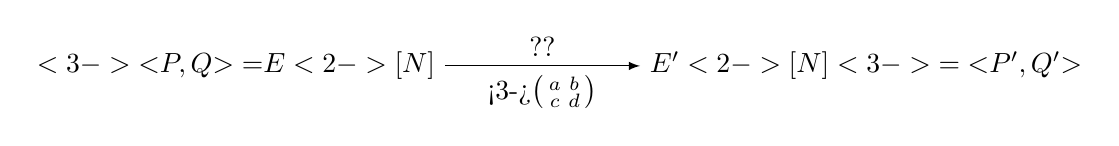
\begin{tikzpicture}[scale=2]
    \node (E) at (0,0) {$\uncover<3->{〈P,Q〉=}E\uncover<2->{[N]}$};
    \node (E1) at (4,0) {$E'\uncover<2->{[N]}\uncover<3->{=〈P',Q'〉}$};
    \draw[-latex] (E) edge node[above] {??} node[below] {{\uncover<3->{$\left(\begin{smallmatrix}a&b\\c&d\end{smallmatrix}\right)$}}} (E1);
  \end{tikzpicture}
\end{frame}

%%

\begin{frame}{Theorem (Robert)}
  \large\centering
  \begin{minipage}{0.8\linewidth}
    Let $E,E'$ be elliptic curves, let \emph{$\phi:E\to E'$} be an
    isogeny of degree \emph{$d$} and let \emph{$N>d$} be an integer
    coprime to $d$.
    
    \bigskip
    
    There exists a polynomial time algorithm that, given
    \emph{$E,E',d,N$}, a basis \emph{$(P,Q)$} of \emph{$E[N]$} and its
    image \emph{$(\phi(P),\phi(Q))$} under $\phi$, computes $\phi$.
  \end{minipage}
\end{frame}

%%

\begin{frame}{$Γ$-SIDH problems}
  \centering
  \large
  Level structure = basis of $E[N]$ up to linear transformations $Γ ⊂ \GL_2(ℤ/N)$

  \vspace{3em}  
  \Large
  \begin{tikzpicture}[scale=2]
    \node (E) at (0,0) {$〈P,Q〉$};
    \node (E1) at (4,0) {$〈P',Q'〉$};
    \draw[-latex] (E) edge node[above] {??}
    node[below] {$\left(\begin{smallmatrix}a&b\\c&d\end{smallmatrix}\right) \uncover<2->{\cdot Γ}$} (E1);
  \end{tikzpicture}
\end{frame}

%%

\begin{frame}{Weil pairing}
  \Large
  \[e_N\bigl(\alert{\phi}(P), \alert{\phi}(Q)\bigr)^{\emph{ad-bc}} =
    e_N(\emph{a}P+\emph{c}Q,\emph{b}P+\emph{d}Q)^{\alert{\deg\phi}}\]
\end{frame}

%%

\begin{frame}{Some examples of level structures}
  \large
  Restricting to $Γ ⊂ \SL_2(ℤ/N)$:
  \bigskip
  \begin{description}
    \setlength{\itemsep}{1em}
  \item[$Γ = \{\left(\begin{smallmatrix}1&\\&1\end{smallmatrix}\right)\}$:]
    A basis $(P,Q)$ of $E[N]$, plain SIDH.
  \item[$Γ = \{\left(\begin{smallmatrix}*&\\&*\end{smallmatrix}\right)\}$:] 
    Two cyclic subgroups $〈P〉$ and $〈Q〉$ of order $N$.
  \item[$Γ_1 = \{\left(\begin{smallmatrix}1&*\\&1\end{smallmatrix}\right)\}$:] 
    A point $P$ of order $N$.
  \item[$Γ_0 = \{\left(\begin{smallmatrix}*&*\\&*\end{smallmatrix}\right)\}$:] 
    A cyclic group $〈P〉$ of order $N$.
  \end{description}
\end{frame}

%%

\begin{frame}{$\{\left(\begin{smallmatrix}*&*\\&*\end{smallmatrix}\right)\}$-SIDH and $\{\left(\begin{smallmatrix}1&*\\&1\end{smallmatrix}\right)\}$-SIDH}
  \large\centering
  \begin{tikzpicture}
    \node at (0,1) {Curve + cyclic subgroup};
    \node at (0,0) {$E, 〈P〉$};
    \node at (4,-.5) {\LARGE$=$};
    \node at (8,1) {Curve + isogeny};
    \node (E) at (8,0) {$E$};
    \node (EP) at (8,-2) {$E/〈P〉$};
    \draw[-latex] (E) edge (EP);
  \end{tikzpicture}
\end{frame}

%%

\begin{frame}{$\{\left(\begin{smallmatrix}*&*\\&*\end{smallmatrix}\right)\}$-SIDH and $\{\left(\begin{smallmatrix}1&*\\&1\end{smallmatrix}\right)\}$-SIDH}
  \large\centering
  \begin{tikzpicture}
    \node (E) at (0,0) {$E$};
    \node (EP) at (0,-2) {$E/〈P〉$};
    \node (E1) at (8,0) {$E'$};
    \node (E1P) at (8,-2) {$E'/〈\phi(P)〉$};
    \draw[-latex] (E) edge (EP) (E1) edge (E1P);
    \draw[dashed,-latex] (E) edge node[above] {$\phi$} (E1);
  \end{tikzpicture}
  
  \vspace{2em} Distinguishing
  $\{\left(\begin{smallmatrix}*&*\\&*\end{smallmatrix}\right)\}$-problem
  aka \emph{Decisional SuperSingular Product (DSSP)}\dots
  
  \bigskip
  \uncover<2->{
    \dots but careful not to reveal $(E,\emph{P},E',\emph{\phi(P)})$ instead!
  }
\end{frame}

%%

\begin{frame}{A reduction {\normalsize(say \emph{$N = n^2$})}}

  \large\centering
  \begin{tikzpicture}
    \node (E) at (0,0) {\alt<1>{$(E,P)$}{$E$}};
    \node (E1) at (8,0) {\alt<1>{$(E',α\phi(P))$}{$E'$}};
    \uncover<-2>{
      \draw[dashed,-latex] (E) edge node[above] {$\phi$} (E1);
    }
    \node[gray] at (12,0) {$\left(\begin{smallmatrix}α&*\\&α^{-1}\end{smallmatrix}\right)$};

    \uncover<2->{
      \node (EnP) at (0,-2) {$E/〈nP〉$};
      \node (EP) at (0,-4) {$E/〈P〉$};
      \node (E1nP) at (8,-2) {$E'/〈nα\phi(P)〉$};
      \node (E1P) at (8,-4) {$E'/〈α\phi(P)〉$};
      
      \uncover<2>{
        \draw[-latex] (E) edge (EnP) (E1) edge (E1nP);
      }
      \uncover<3->{
        \draw[latex-] (E) edge (EnP) (E1) edge (E1nP);
      }
      \draw[-latex] (EnP) edge (EP) (E1nP) edge (E1P);
    }

    \uncover<3-> {
      \draw[dashed,-latex] (EnP) edge node[above] {$\phi'$} (E1nP);
      \node[gray] at (12,-2) {$\left(\begin{smallmatrix}α&n*\\n*&α^{-1}\end{smallmatrix}\right)$};
    }

    \uncover<4->{
      \node[gray] at (12,-3) {$=\left(\begin{smallmatrix}α&\\&α^{-1}\end{smallmatrix}\right) \mod n$};
    }
  \end{tikzpicture}  
\end{frame}

%%

\begin{frame}{A reduction}
  \Large\centering
  \begin{tikzpicture}[x=1.5cm,scale=2]
    \node (SIDH) at (0,0) {SIDH};
    \node (MSIDH) at (1,-1) {$\sm{\lambda&}{&\lambda}$};
    \node (DIAG) at (1,-2) {$\sm{*&}{&*}$};
    \node (UNI) at (-1,-1.5) {$\sm{1&*}{&1}$};
    \node (HECKE) at (0,-3) {$\sm{*&*}{&*}$};

    \draw[gray,-latex] (SIDH) edge (MSIDH) edge (UNI)
    (UNI) edge (HECKE)
    (MSIDH) edge (DIAG)
    (DIAG) edge (HECKE);

    \draw[dashed,->] (UNI) edge[bend left] (SIDH)
    (HECKE) edge[bend right] (DIAG);

    \draw[dotted,->] (MSIDH) edge[bend right] (SIDH);
  \end{tikzpicture}
\end{frame}

%%

\begin{frame}{$\sm{λ}{&λ}$-SIDH}
  \centering\large
  Harder than SIDH when $N$ has many prime factors?

  \vspace{2em}
  See \emph{Fouotsa, Moriya, Petit -- Eurocrypt 2023}.
\end{frame}

%% 

\begin{frame}{CSIDH $\to \sm{*}{&*}$-SIDH}
  \centering\large

  \begin{tikzpicture}
    \node (E) at (0,0) {$E$};
    \node (E1) at (8,0) {$E'$};
    \draw[dashed,-latex] (E) edge node[above] {$\phi$} (E1);
    \draw[gray]
    (E) edge[loop above] node[above] {$π$} (E)
    (E1) edge[loop above] node[above] {$π'$} (E1);

    \uncover<2->{
      \node at (0,-1) {$π|〈P,Q〉 = \sm{λ}{&-λ}$};
      \node at (8,-1) {$π'|〈P',Q'〉 = \sm{λ}{&-λ}$};
    }
  \end{tikzpicture}

  \vspace{2em}
  \uncover<2->{
    Frobenius diagonalizes on $E[N]$ for every prime $N$
    s.t. $\left(\frac{-p}{N}\right) = 1$.
  }
\end{frame}

%% 

\begin{frame}
  \centering
  \begin{tikzpicture}
    \draw[gray,-latex] (-.2,-.2) -- (-.2,7);
    \node[anchor=center] at (-2.4,3) {\parbox{5em}{\centering Torsion knowledge}};
    \draw[gray,anchor=east,font=\small,shift={(-.2,0)}]
    (0,0) -- +(-.1,0) node {None}
    (0,2.5) -- +(-.1,0) node {$\left(\begin{smallmatrix}*&*\\&*\end{smallmatrix}\right)$}
    (0,3.5) -- +(-.1,0) node {$\left(\begin{smallmatrix}*&\\&*\end{smallmatrix}\right)$}
    (0,4.5) -- +(-.1,0) node {$\left(\begin{smallmatrix}λ&\\&λ\end{smallmatrix}\right)$}
    (0,5) -- +(-.1,0) node {$\left(\begin{smallmatrix}1&*\\&1\end{smallmatrix}\right)$}
    (0,6) -- +(-.1,0) node {Full};
    
    \draw[gray,-latex] (-.2,-.2) -- (12,-.2);
    \node[anchor=center] at (6,-1.2) {$\End(E)$ knowledge};
    \draw[gray,anchor=north,font=\small,shift={(0,-.2)}]
    (0,0) -- +(0,-.1) node {None}
    (5.5,0) -- +(0,-.1) node {Orientation}
    (11,0) -- +(0,-.1) node {Full};

    \begin{uncoverenv}<2->
      \small
      \draw[green!50!black] (0,0) node {$\bullet$} node[anchor=south west] {SQISign};
      \draw[green!50!black] (0,2.5) node {$\bullet$} node[anchor=west] {\parbox{8em}{\centering SIDH signatures (DSSP)}};
      \draw[green!50!black] (0,4.5) node {$\bullet$} node[anchor=west] {M-SIDH};
      \draw[red] (0,6) node {$\times$} node[anchor=north west] {SIDH};
      \draw[red] (11,0) node {$\times$} node[anchor=south east] {\parbox{9em}{\centering Eisenträger et al. '18\\Wesolowski '21}};
      \draw[orange] (5.5,3.5) node {$\bullet$} node[anchor=north] {\parbox{5em}{\centering CSIDH\\SCALLOP}};
      
      \fill[pattern=north west lines,pattern color=red] (1,5.8) -- ++(0,.4) -- ++(10.2,0) -- ++(0,-5.2) -- ++(-.4,0) -- ++(0,4.8);
      \fill[pattern=north west lines,pattern color=gray] (5,-.2) -- ++(1,0) -- ++(0,1) -- ++(-1,0);
    \end{uncoverenv}

    \begin{uncoverenv}<2->
      \draw[<->] (-.8,2.8) -- +(0,.4);
      \draw[<->] (-.8,5.3) -- +(0,.4);
      \draw[dashed,orange] (6.5,-.4) edge[->] node[below] {\tiny quantum subexp} +(4,0);
    \end{uncoverenv}
  \end{tikzpicture}
\end{frame}

%%

\begin{frame}[plain]
  \centering
  \begin{tikzpicture}[remember picture,overlay]
    \begin{scope}[xscale=1.7,yshift=-15,opacity=0.8]
      \def\crater{12}
      \def\jumpa{-8}
      \def\jumpb{9}
      \def\diam{5cm}

      \foreach \i in {1,...,\crater} {
        \draw[blue] (360/\crater*\i : \diam) to[bend right] (360/\crater*\i+360/\crater : \diam);
        \draw[red] (360/\crater*\i : \diam) to[bend right] (360/\crater*\i+\jumpa*360/\crater : \diam);
        \draw[green] (360/\crater*\i : \diam) to[bend right=50] (360/\crater*\i+\jumpb*360/\crater : \diam);
      }
    \end{scope}
    
    \draw (0,0.5) node{\Huge\bf Thank you};
    \draw (0,-0.6) node{\large\url{https://defeo.lu/}};
    \draw (0,-1.3) node{\large\includegraphics[height=0.9em]{mastodon.png}~\href{https://twitter.com/luca_defeo}{@luca\_defeo@ioc.exchange}};
    \draw (0,-1.9) node{\large\includegraphics[height=0.9em]{twitter.png}~\href{https://twitter.com/luca_defeo}{@luca\_defeo}};
  \end{tikzpicture}
\end{frame}

%%

\end{document}


% LocalWords:  Isogeny abelian isogenies hyperelliptic supersingular Frobenius
% LocalWords:  isogenous
